\definecolor{lavander}{cmyk}{0,0.48,0,0}
\definecolor{violet}{cmyk}{0.79,0.88,0,0}
\definecolor{burntorange}{cmyk}{0,0.52,1,0}

\def\lav{lavander!90}
\def\oran{orange!30}

\tikzstyle{contingency}=[draw,circle,violet,bottom color=\lav,
                  top color= white, text=violet,minimum width=20pt]
\tikzstyle{base}=[draw,circle,burntorange, left color=\oran,
                       text=violet,minimum width=20pt]
                       
\tikzstyle{cedge}=[color=red]

\begin{figure}[h!]
\centering
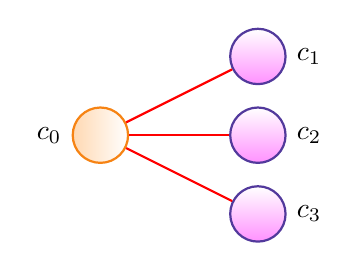
\begin{tikzpicture}[auto, thick]
  % Place base case
  \node[base,label=left:$c_0$] (base) at (0,0) {};
  
  \node[contingency,label=right:$c_1$] (c1) at (2,1) {};
  \node[contingency,label=right:$c_2$] (c2) at (2,0) {};
  \node[contingency,label=right:$c_3$] (c3) at (2,-1) {};
  
  \path[cedge] (base) edge (c1);
  \path[cedge] (base) edge (c2);
  \path[cedge] (base) edge (c3);
  
  
  
%  \foreach \place/\name in {{(0,-1)/a}, {(2,0)/b}, {(2,2)/c}, {(0,2)/d},
%           {(-2,0)/e}}
%    \node[superpeers] (\name) at \place {a};
%  \foreach \source/\dest in {a/b, a/c, a/d, b/c, c/d,a/e,d/e}
%    \path (\source) edge (\dest);
   %
   % Place normal peers
%  \foreach \pos/\i in {above left of/1, left of/2, below left of/3}
%    \node[peers, \pos = e] (e\i) {};
%   \foreach \speer/\peer in {e/e1,e/e2,e/e3}
%    \path (\speer) edge (\peer);
   %
%   \foreach \pos/\i in {above right of/1, right of/2, below right of/3}
%    \node[peers, \pos =b ] (b\i) {};
%   \foreach \speer/\peer in {b/b1,b/b2,b/b3}
%   \path (\speer) edge (\peer);
   %
%   \node[peers, above of=d] (d1){};
%   \path (d) edge (d1);
   %
%   \foreach \pos/\i in {below left of/1, below of/2}
%   \node[peers, \pos =a ] (a\i) {};
%   \foreach \speer/\peer in {a/a1,a/a2}
%   \path (\speer) edge (\peer);

\end{tikzpicture}
\caption{Contingency constrained optimal power flow example with three contingencies. $c_0$ represents the base case (or no contingency case). $c_1$, $c_2$, $c_3$ are the three contingency cases. Each of the contingency states is coupled with the base-case through ramping constraints (denoted by \textcolor{red}{red} lines)}
\label{fig:scopflow}
\end{figure}
